\section{Adapting STEGO for Scientific Images}\label{sec:adapting-stego}
As mentioned before, \gls{stego} needed some adaptions to be used with 3D high-resolution scientific images.
This comprised correcting and refactoring the code to make it executable, setting all the configuration variables to the optimal values as found by the authors or according to the data set used for training, and also adapting \gls{stego} to be used with high-resolution grey value images, since the expected inputs were 2D RGB color photographs.~\autocite{Hamilton2022}


\subsection{Code Refactoring and Corrections}
%configuration files
Since the code base of \gls{stego} was very much the raw project, which contains all experiments presented in~\autocite{Hamilton2022}, there were a lot of configuration variables present. 
For these the optimal values often have been already found by the authors, so they were not needed anymore or best set to a predefined value.
Moreover, the provided configuration files were often not used consistently in the executable scripts.
Frequently, the configuration parameters from the configuration files were overwritten with hardcoded values in the executable files.
Overall, these problems could be solved by replacing all the hardcoded parameters with parameters from the configuration file first and then investigating which configuration variable belonged to which part of the experiments mentioned in the paper (since they were not documented at all).
Finally, the configuration file structure was adapted to a hierarchy, so it was easier to distinguish between parameters to define the backbone, parameters to control training, and parameters for selected data sets.

% fixes during training
The training procedure did only work for the provided example datasets and not for own datasets (directory datasets), since during the validation, label names are required, which were again hardcoded for the example datasets, but of course not available for directory datasets.
This was solved by adding a labels parameter to the configuration file, which is read when own datasets are trained.
Calculation of the nearest neighbours of an image was changed to read the images in the given resolution, instead of using the hardcoded (down-scaled) size, since it is expected that better matching neighbours will be found.

% fixes during validation
Other fixes were needed during validation when creating diagnostic pictures, since the label number was calculated incorrectly when extra clusters were used.
Additionally, the label tensor made during training needed squeezing in order to be passed to the plotting function during validation (so some example predictions can be plotted to illustrate the training progress via \tensorboard).
Lastly, loading of the validation images was changed to always load the original validation images (of the un-cropped dataset), since loading the down-scaled images would provide only very weak evidence on model improvement.
Additionally, resolution and batch size of the validation set was adapted to be selected independently of the train set, so the validation images can be interpreted easier. 

% `fixes' during evaluation
The evaluation procedure used by the authors focused on comparing \gls{stego} with the former state of the art for unsupervised segmentation (PiCIE~\autocite{Cho2021}), so new evaluation scripts were made to evaluate a trained model based on a test set.\footnote{With the new evaluation script, evaluations can be done by running the model on a test set belonging to the data set the model was trained on or by giving a path to the image and ground truth folder to be used for evaluation.}
During evaluation, \gls{miou} and accuracy for the test set are reported, as well as some diagnostic graphs, to show correlation between ground truth labels and predicted labels, as well as to display some example segmentations side by side with their ground truth and original image.

% cosmetic corrections (refactoring)
Additionally, some non-functional alterations were made:
\begin{itemize}
    %\item Repaired issue with the evaluation script not showing a progress bar by fixing multiprocessing.
    \item For better adaptability and easier way of training on different data sets, the configuration file structure was adjusted, so that for every script, the base configurations are collected in one configuration file, while all data set specific configurations are collected in a separate file, which is selected via the command line for each training separately.
    \item The output directories were changed to depend on the output path given in the configuration, instead of saving everything in the code folder.
    \item For better comprehension and clearer view on what is happening in the code, the full configurations are no longer passed between scripts, only the relevant variables extracted from the configuration will be passed.
    \item The code was also adjusted to get rid of warnings of future deprecations, since the provided conda environment specified some very particular, but often older versions for packages.\footnote{As it was found that updating \gls{stego} to other Python versions leads to problems during training, it was decided to not change the suggested conda environment.}
    Note, that not all warnings have been resolved.
\end{itemize} 

%Things that should be changed, but weren't:
Due to time constraints, some issues have not been addressed, since they do not influence results, but mainly user experience.
For a full list see~\autoref{subsec:stego-persisting-issued}.


\subsection{Adaption to High-resolution Grey Value Images}
\gls{stego} was designed with photographs in mind.
Thus, some adaptions needed to be made to use it with scientific images, mainly to adjust the normalisation scheme to grey values, load high-resolution images and handle 3D images.
In the following, these changes are documented, always in relation to the original architecture~\autocite{Hamilton2022}.

The more simple adaption concerned the normalisation scheme during preprocessing, when a pixel value normalisation for each channel was done, based on the mean and standard deviation of the ImageNet data set\footnote{https://www.image-net.org/ (visited 15/02/2023)}.
The different normalisation of the three RGB channels was of course not appropriate for images that represent grey values.
Thus, in the configurations file used for training, a flag was added to indicate if images are grey values and in \gls{stego}, a normalisation function based on the grey value of ImageNet pictures was added.

Another problem was the scaling \gls{stego} applies when loading images.
Since often images could not be loaded at full resolution, all images were scaled to the user-defined resolution.
For scientific data, this means a lot of the cumbersome earned and probably relevant details would be lost.
Thus, a second flag was added in the configuration file to switch between down-scaling and center-cropping the loaded images to size.
Of course, this way some data is still lost, but instead of loosing overall details, now the borders of the images are missing, which are often not the regions of interest.
Overall, establishing the possibility to crop instead of scale means, that in combination with five-cropping and selecting an appropriate resolution, the maximal amount of relevant details of the images can be utilised with \gls{stego}.

For a more fine-grained evaluation, \gls{stego} was also adapted, to display the label-wise \gls{iou} (additional to the mean over labels) in the \tensorboard to better understand how individual labels perform.
This change did not alter the architecture significantly, since these values could be simply extracted before the mean was calculated.


\gls{stego} originally was developed to train and predict 2D photographs.
To use it with 3D data, the volumes need to be sliced into a stack of 2D images (and reassembled later on).
Therefore, a data converter was designed, which converts the in-house data sets to the required format.
However, data conversion is done separately from \gls{stego} and thus not part of this project.

\begin{figure}[!htb]
    \centering
    \vspace{1em}
    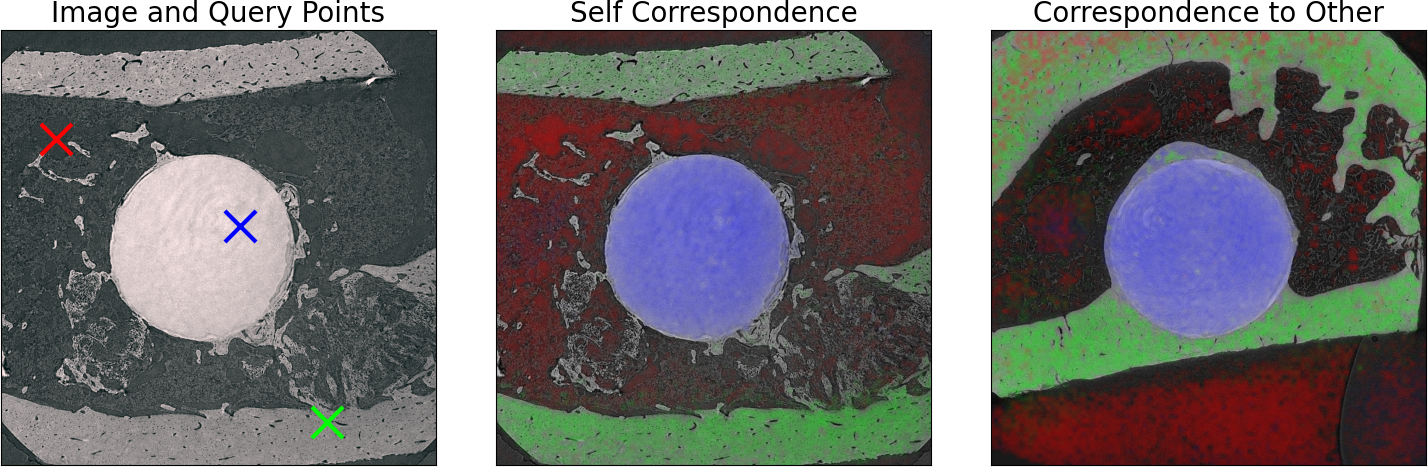
\includegraphics[width=\textwidth]{pictures/correspondencemaps_syn030-slice300_113724Mg10-slice500}\\
    \caption[Feature Correspondence for SRµCT Images]{Feature correspondences maps for SRµCT images derived from the DINO-backbone of \gls{stego}. Correspondences for selected points (marked with x) are plotted over the same (middle) and another target image (right) in the respective color of the source point.}
    \label{fig:correspondencemap-screws}
\end{figure}

It was decided to use the frozen backbone that was trained on photographs too, since investigating exemplary attention maps showed, that this backbone is already able to indicate correspondences from \gls{srmct} images, as seen in~\autoref{fig:correspondencemap-screws}.
This can be interpreted as a form of transfer learning~\autocite{Litjens2017}, which yields promising results in some cases, as networks trained exactly on this data set have been found to yield good results when used with medical images as well (for an overview on performance of transfer learning, see~\autocite{Cheplygina2019}).










